\documentclass[%
    reprint,
    onecolumn,
    nofootinbib,
    amsmath,
    amssymb,
    aps,
    prstab,
]{revtex4-2}

\usepackage{graphicx} 

\begin{document}


\title{Supplementary Material for ``High-dimensional maximum-entropy phase space tomography using normalizing flows''}


\maketitle

The following figures repeat the numerical experiment in Fig.2 of the main text for different ground-truth distributions.

%
\begin{figure*}
    \centering
    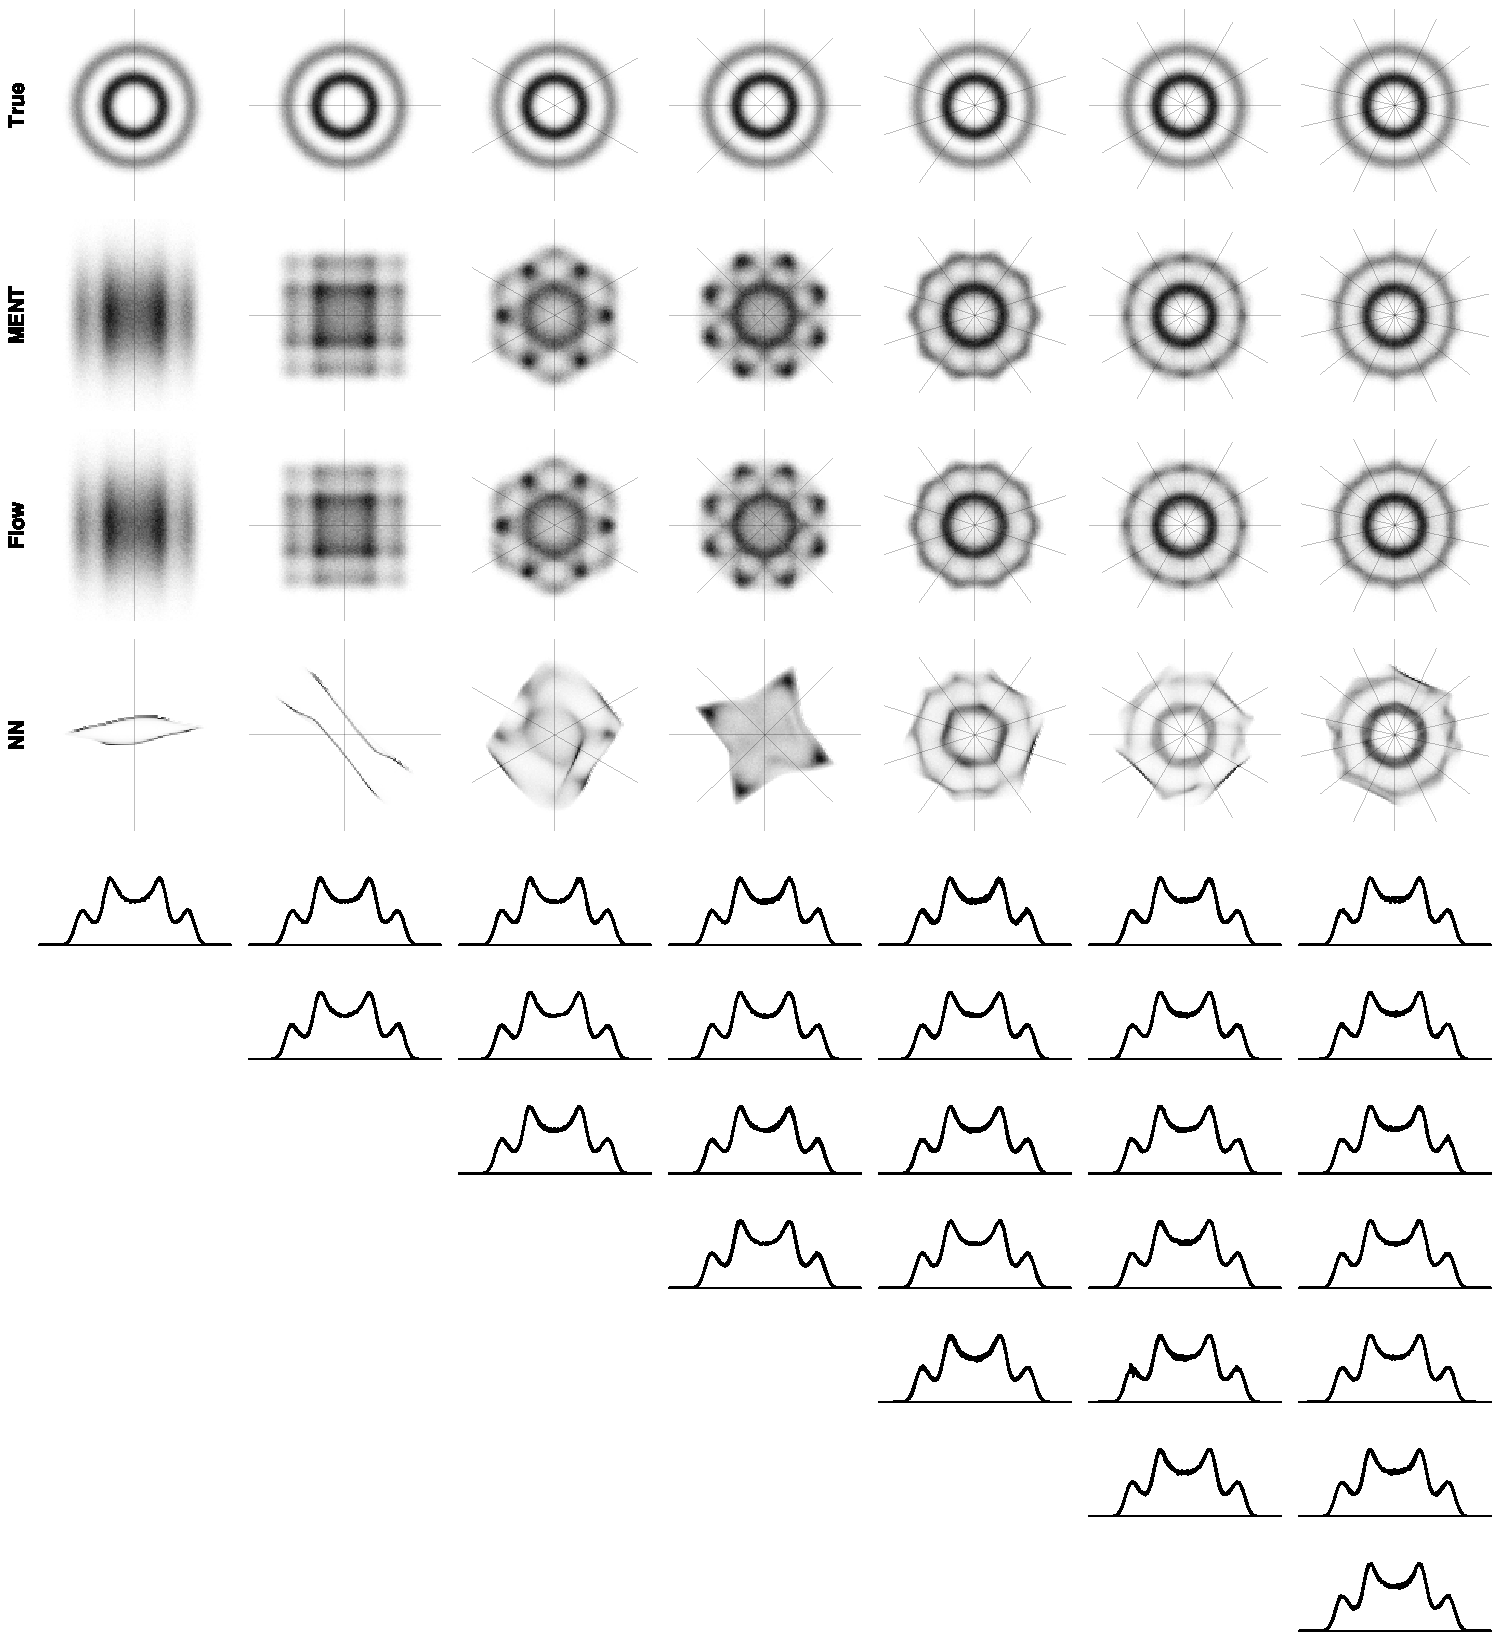
\includegraphics[width=\textwidth]{fig_rec_2d_rings.pdf}
    \caption{2D reconstruction of the ``rings'' distribution from evenly spaced 1D projections. The top four rows plot samples from the true distribution, MENT reconstruction, MENT-Flow reconstruction, and NN reconstruction. Faint lines show the evenly spaced projection angles, increasing from 1 in the left column to 7 in the right column. In the bottom rows, the distributions are projected onto the measurement axes. (The four profiles overlap in most cases.)}
    \label{fig:rec_2d_rings}
\end{figure*}
%
%
\begin{figure*}
    \centering
    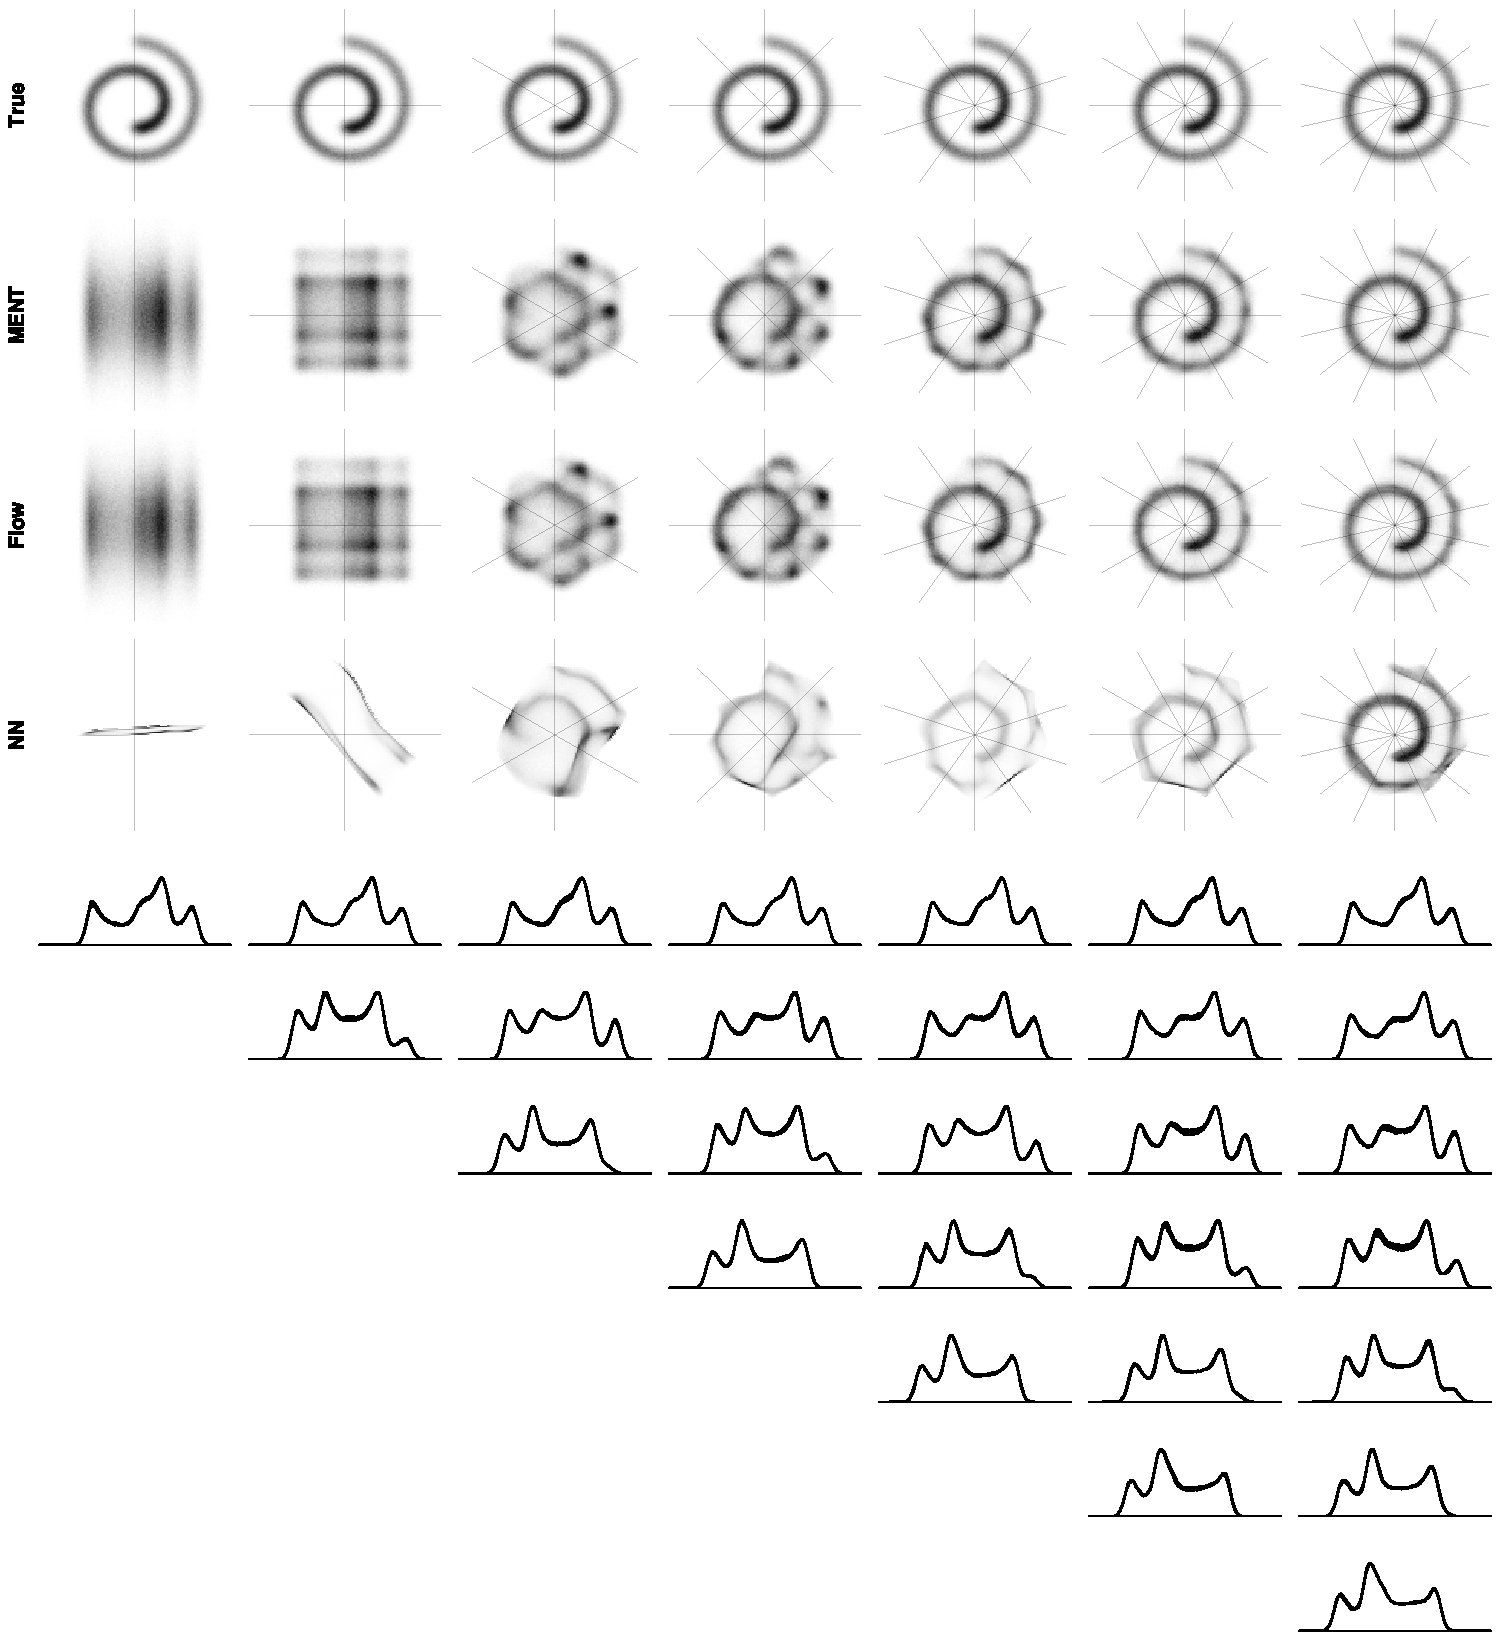
\includegraphics[width=\textwidth]{fig_rec_2d_swissroll.pdf}
    \caption{2D reconstruction of the ``swissroll'' distribution from evenly spaced 1D projections. The top four rows plot samples from the true distribution, MENT reconstruction, MENT-Flow reconstruction, and NN reconstruction. Faint lines show the evenly spaced projection angles, increasing from 1 in the left column to 7 in the right column. In the bottom rows, the distributions are projected onto the measurement axes. (The four profiles overlap in most cases.)}
    \label{fig:rec_2d_swissroll}
\end{figure*}
%
%
\begin{figure*}
    \centering
    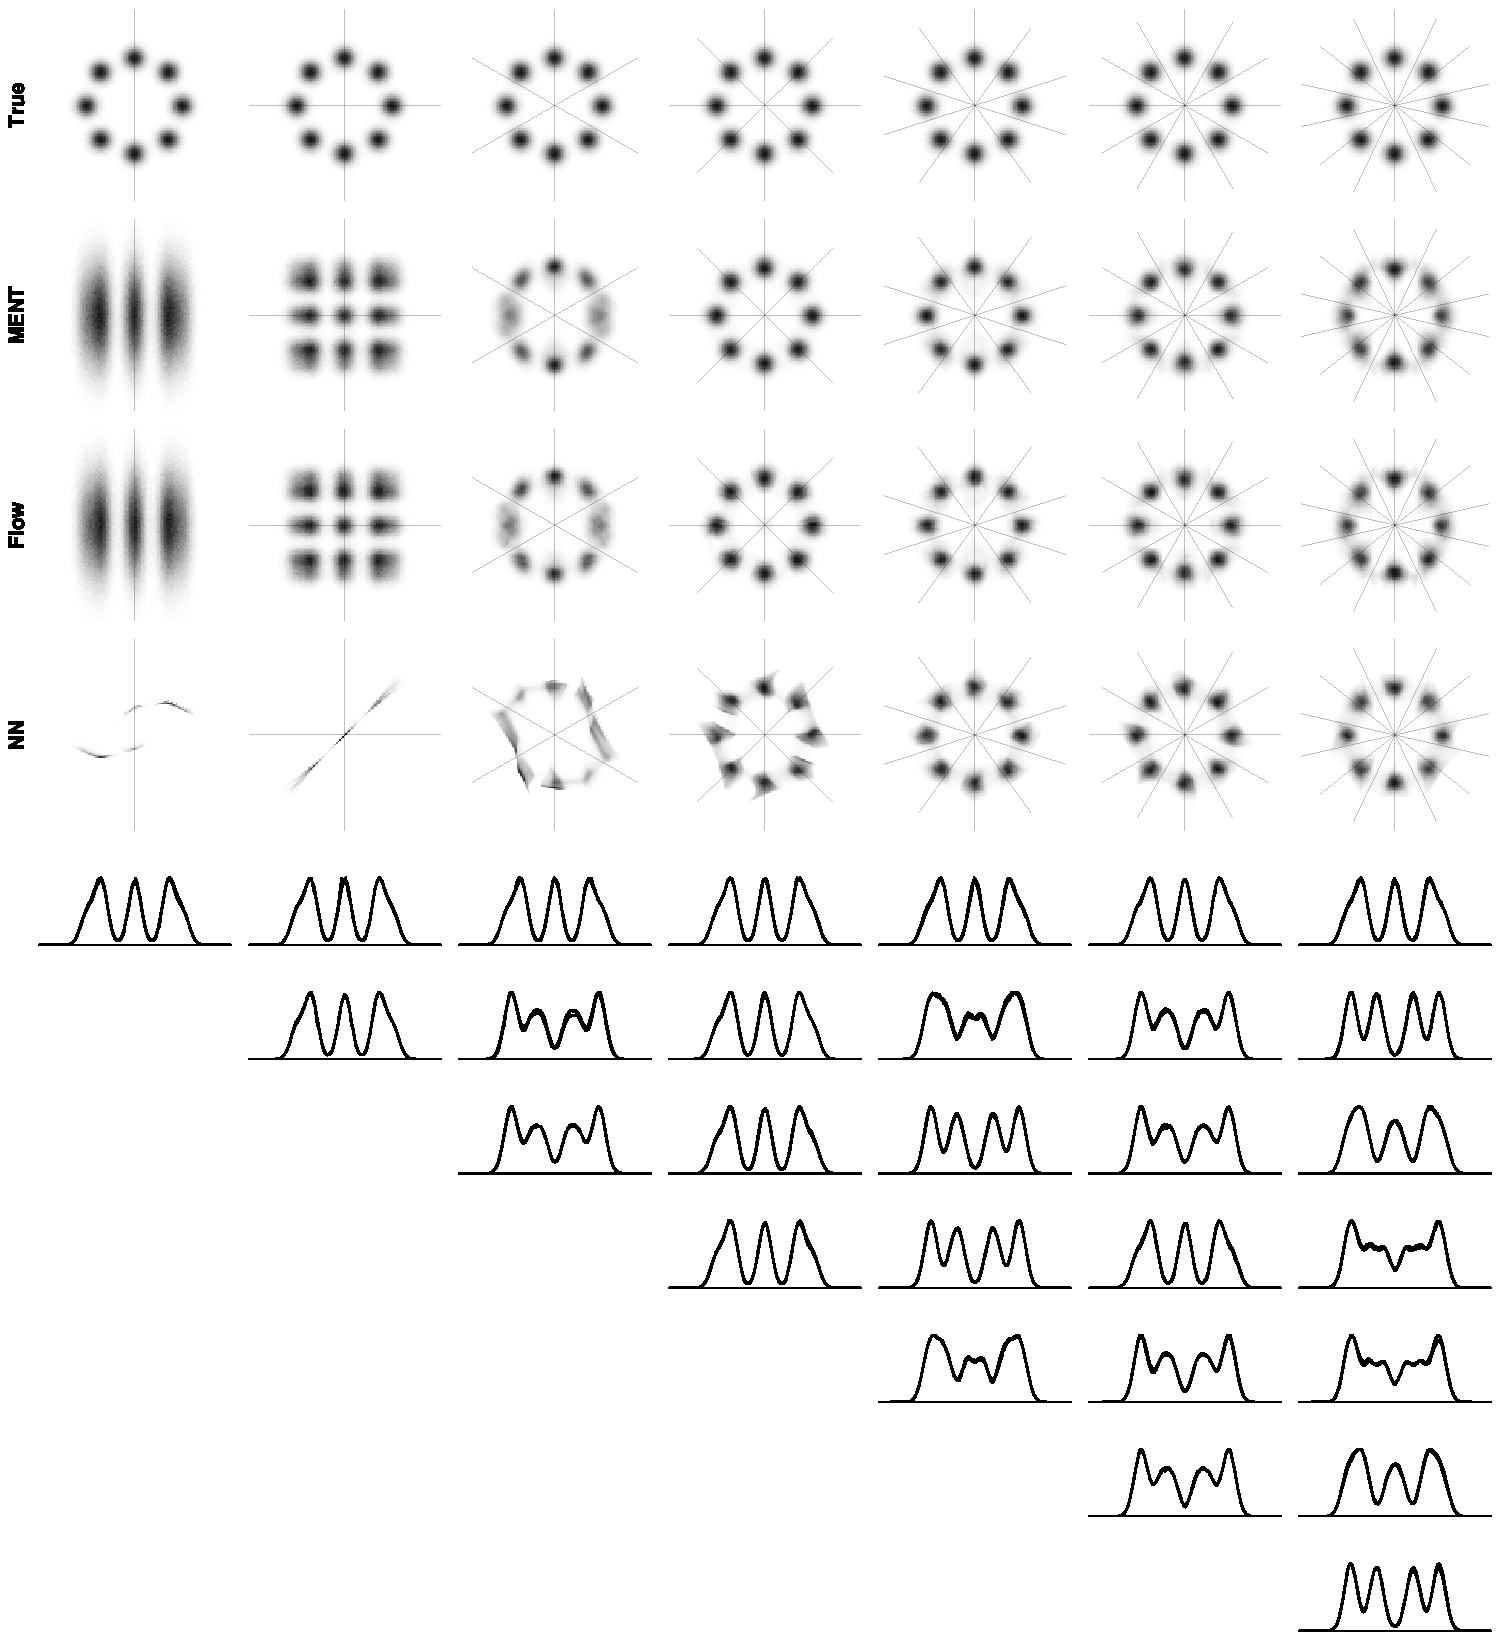
\includegraphics[width=\textwidth]{fig_rec_2d_eight-gaussians.pdf}
    \caption{2D reconstruction of the ``eight gaussians'' distribution from evenly spaced 1D projections. The top four rows plot samples from the true distribution, MENT reconstruction, MENT-Flow reconstruction, and NN reconstruction. Faint lines show the evenly spaced projection angles, increasing from 1 in the left column to 7 in the right column. In the bottom rows, the distributions are projected onto the measurement axes. (The four profiles overlap in most cases.)}
    \label{fig:rec_2d_eight-gaussians}
\end{figure*}
%
%
\begin{figure*}
    \centering
    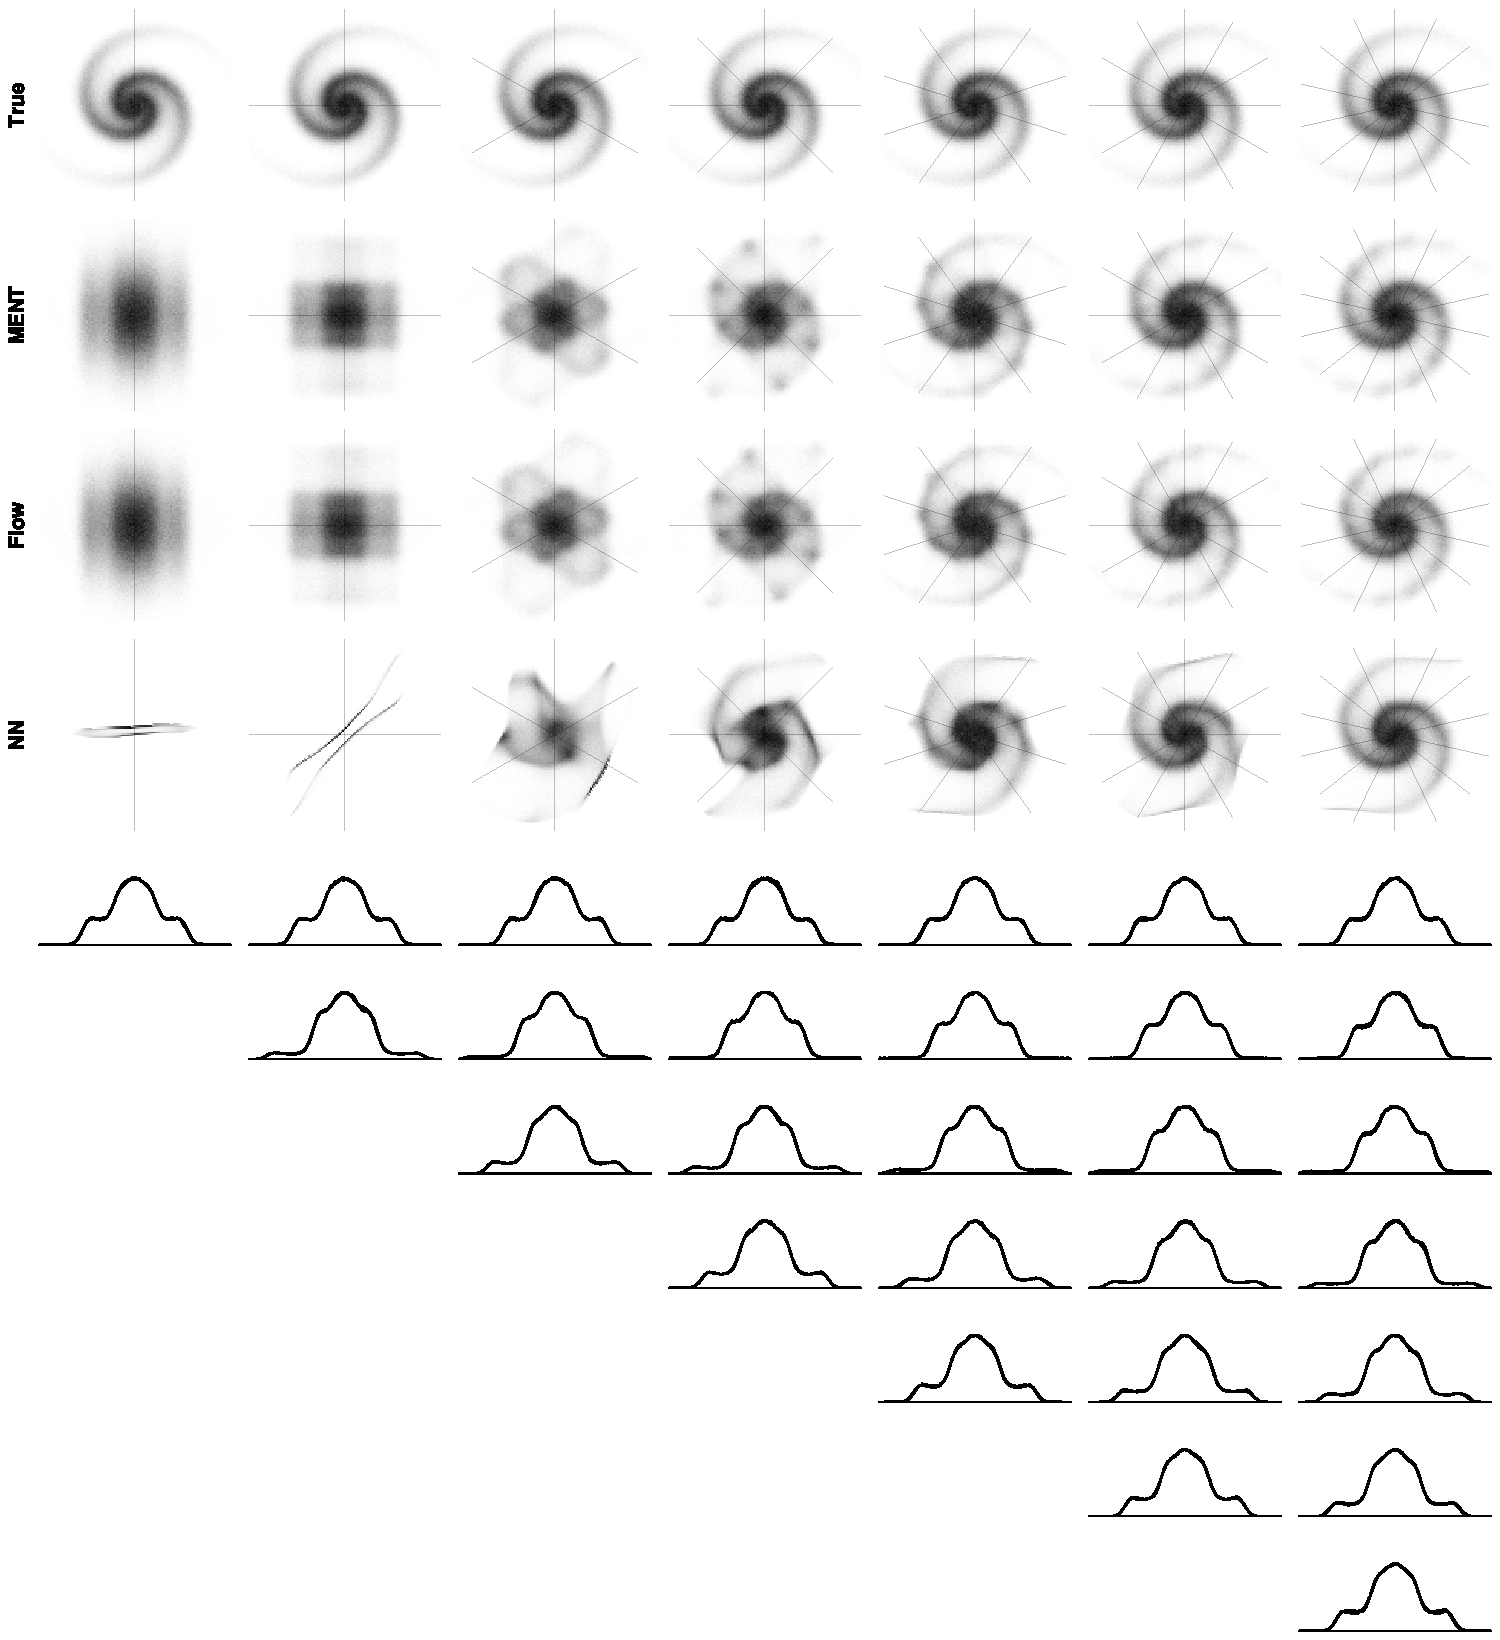
\includegraphics[width=\textwidth]{fig_rec_2d_galaxy.pdf}
    \caption{2D reconstruction of the ``galaxy'' distribution from evenly spaced 1D projections. The top four rows plot samples from the true distribution, MENT reconstruction, MENT-Flow reconstruction, and NN reconstruction. Faint lines show the evenly spaced projection angles, increasing from 1 in the left column to 7 in the right column. In the bottom rows, the distributions are projected onto the measurement axes. (The four profiles overlap in most cases.)}
    \label{fig:rec_2d_galaxy}
\end{figure*}
%
%
\begin{figure*}
    \centering
    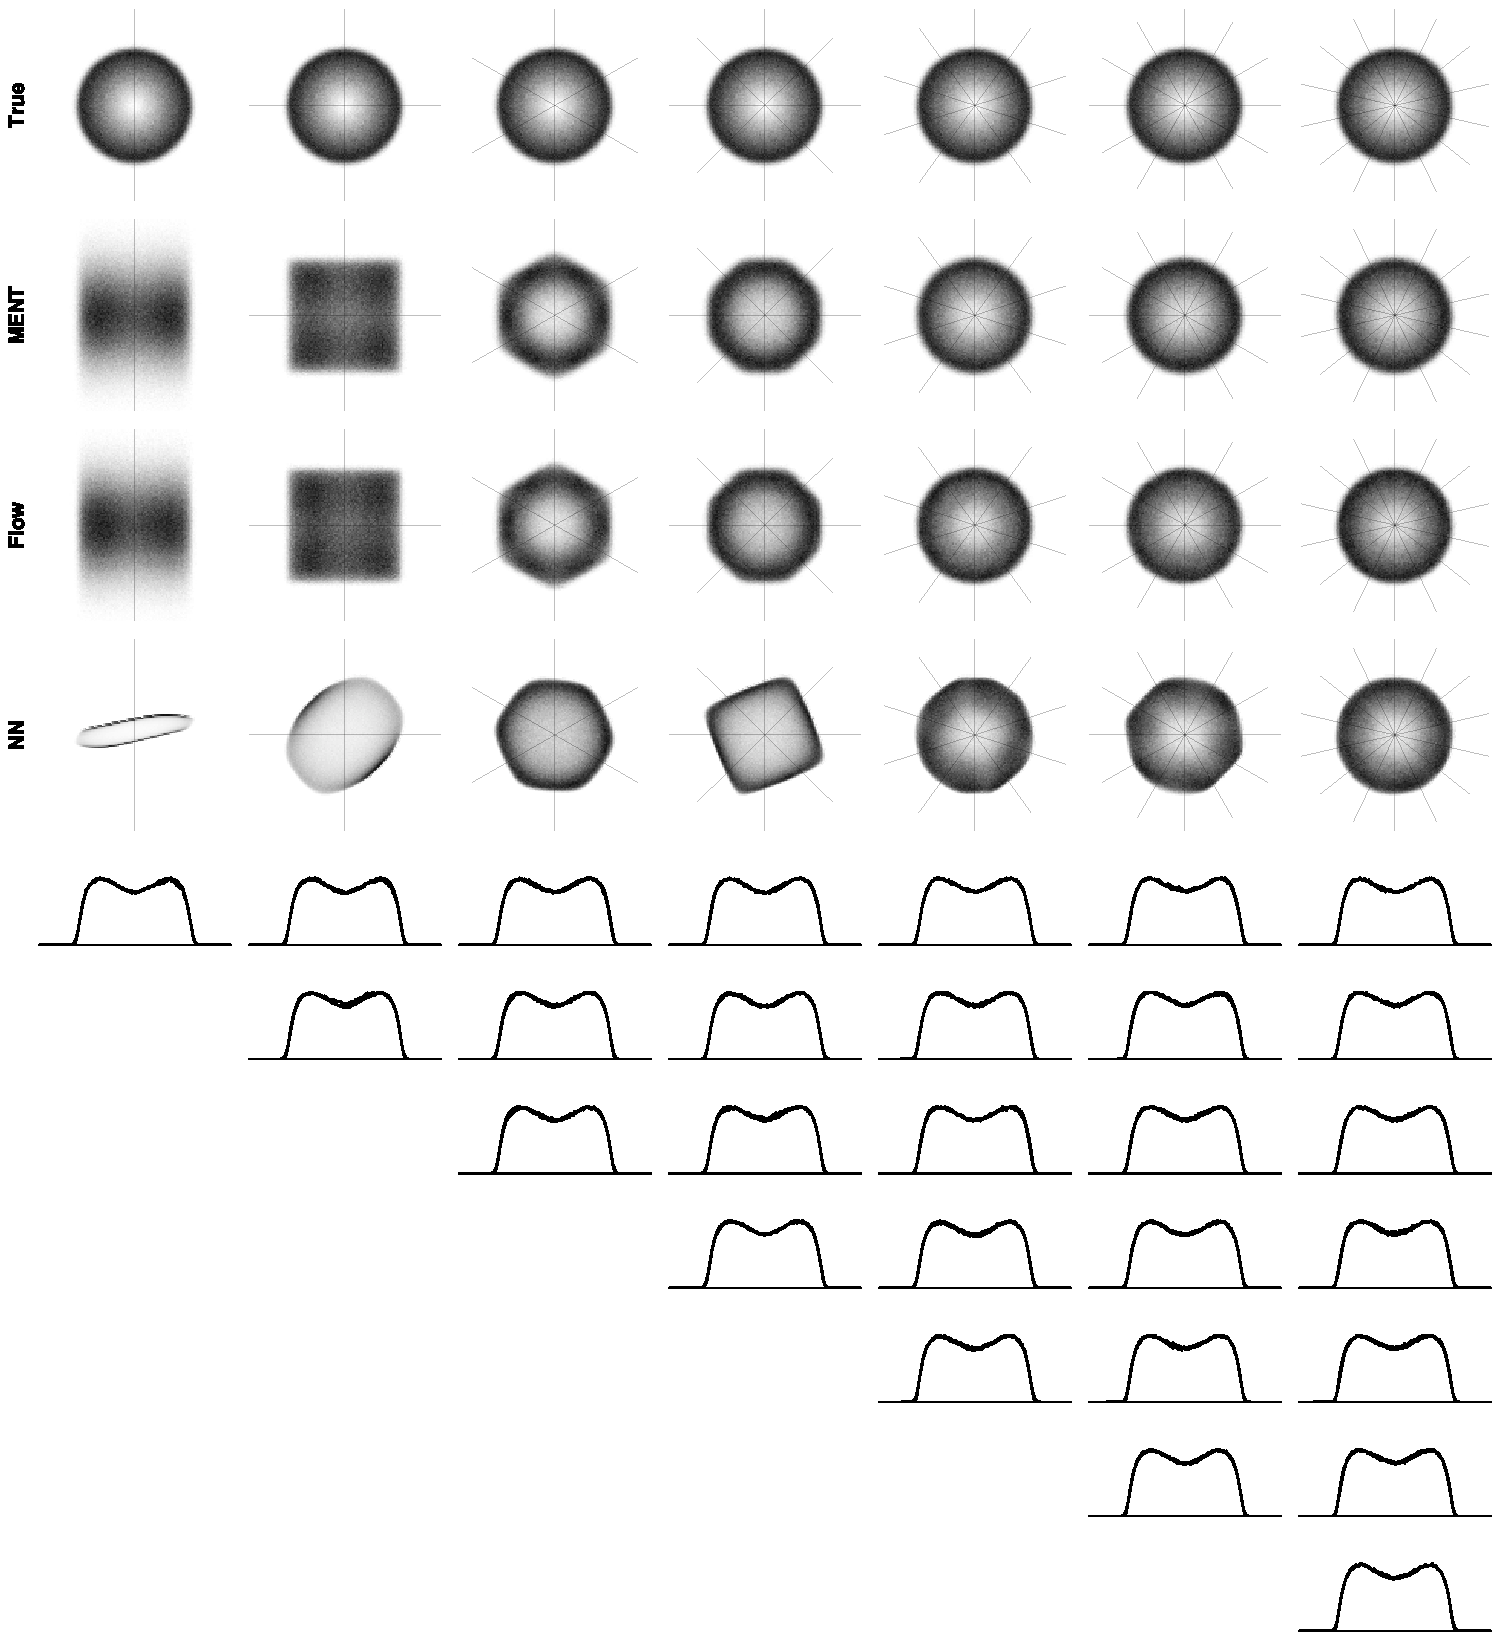
\includegraphics[width=\textwidth]{fig_rec_2d_hollow.pdf}
    \caption{2D reconstruction of the ``hollow'' distribution from evenly spaced 1D projections. The top four rows plot samples from the true distribution, MENT reconstruction, MENT-Flow reconstruction, and NN reconstruction. Faint lines show the evenly spaced projection angles, increasing from 1 in the left column to 7 in the right column. In the bottom rows, the distributions are projected onto the measurement axes. (The four profiles overlap in most cases.)}
    \label{fig:rec_2d_galaxy}
\end{figure*}
%


\end{document}
